\documentclass[12pt]{article}\usepackage[]{graphicx}\usepackage[]{color}
%% maxwidth is the original width if it is less than linewidth
%% otherwise use linewidth (to make sure the graphics do not exceed the margin)
\makeatletter
\def\maxwidth{ %
	\ifdim\Gin@nat@width>\linewidth
	\linewidth
	\else
	\Gin@nat@width
	\fi
}
\makeatother

\definecolor{fgcolor}{rgb}{0.345, 0.345, 0.345}
\newcommand{\hlnum}[1]{\textcolor[rgb]{0.686,0.059,0.569}{#1}}%
\newcommand{\hlstr}[1]{\textcolor[rgb]{0.192,0.494,0.8}{#1}}%
\newcommand{\hlcom}[1]{\textcolor[rgb]{0.678,0.584,0.686}{\textit{#1}}}%
\newcommand{\hlopt}[1]{\textcolor[rgb]{0,0,0}{#1}}%
\newcommand{\hlstd}[1]{\textcolor[rgb]{0.345,0.345,0.345}{#1}}%
\newcommand{\hlkwa}[1]{\textcolor[rgb]{0.161,0.373,0.58}{\textbf{#1}}}%
\newcommand{\hlkwb}[1]{\textcolor[rgb]{0.69,0.353,0.396}{#1}}%
\newcommand{\hlkwc}[1]{\textcolor[rgb]{0.333,0.667,0.333}{#1}}%
\newcommand{\hlkwd}[1]{\textcolor[rgb]{0.7te37,0.353,0.396}{\textbf{#1}}}%

\usepackage{framed}
\makeatletter
\newenvironment{kframe}{%
	\def\at@end@of@kframe{}%
	\ifinner\ifhmode%
	\def\at@end@of@kframe{\end{minipage}}%
\begin{minipage}{\columnwidth}%
	\fi\fi%
	\def\FrameCommand##1{\hskip\@totalleftmargin \hskip-\fboxsep
		\colorbox{shadecolor}{##1}\hskip-\fboxsep
		% There is no \\@totalrightmargin, so:
		\hskip-\linewidth \hskip-\@totalleftmargin \hskip\columnwidth}%
	\MakeFramed {\advance\hsize-\width
		\@totalleftmargin\z@ \linewidth\hsize
		\@setminipage}}%
{\par\unskip\endMakeFramed%
	\at@end@of@kframe}
\makeatother

\definecolor{shadecolor}{rgb}{.97, .97, .97}
\definecolor{messagecolor}{rgb}{0, 0, 0}
\definecolor{warningcolor}{rgb}{1, 0, 1}
\definecolor{errorcolor}{rgb}{1, 0, 0}
\newenvironment{knitrout}{}{} % an empty environment to be redefined in TeX

\usepackage{alltt} % use larger type; default would be 10pt

\usepackage[T5]{fontenc}
\usepackage[utf8]{inputenc} % set input encoding (not needed with XeLaTeX)

%%% Examples of Article customizations
% These packages are optional, depending whether you want the features they provide.
% See the LaTeX Companion or other references for full information.

%%% PAGE DIMENSIONS
\usepackage{geometry} % to change the page dimensions
\geometry{letterpaper} % or letterpaper (US) or a5paper or....
\geometry{margin=1.2in} % for example, change the margins to 2 inches all round
% \geometry{landscape} % set up the page for landscape
%   read geometry.pdf for detailed page layout information

\usepackage{graphicx} % support the \includegraphics command and options

% \usepackage[parfill]{parskip} % Activate to begin paragraphs with an empty line rather than an indent

%%% PACKAGES
\usepackage{booktabs} % for much better looking tables
\usepackage{array} % for better arrays (eg matrices) in maths
\usepackage{paralist} % very flexible & customisable lists (eg. enumerate/itemize, etc.)
\usepackage{verbatim} % adds environment for commenting out blocks of text & for better verbatim
\usepackage{subfig} % make it possible to include more than one captioned figure/table in a single float
\usepackage{setspace}
\usepackage{pdflscape}
\usepackage{amsmath}
\usepackage{url}
\usepackage{multirow}
\usepackage{listings}
\usepackage{dcolumn}
%\usepackage[nolists]{endfloat}
\usepackage{bbm}
\usepackage{pdflscape}
\usepackage{pdfpages}

\usepackage{natbib}
\bibliographystyle{apsr}
\usepackage{hyperref}

%%% HEADERS & FOOTERS
\usepackage{fancyhdr} % This should be set AFTER setting up the page geometry
\pagestyle{fancy} % options: empty , plain , fancy
\renewcommand{\headrulewidth}{0pt} % customise the layout...
\lhead{}\chead{}\rhead{}
\lfoot{}\cfoot{\thepage}\rfoot{}

%%% SECTION TITLE APPEARANCE
\usepackage{sectsty}
\allsectionsfont{\sffamily\mdseries\upshape} % (See the fntguide.pdf for font help)
% (This matches ConTeXt defaults)

%%% ToC (table of contents) APPEARANCE
\usepackage[nottoc,notlof,notlot]{tocbibind} % Put the bibliography in the ToC
\usepackage[titles,subfigure]{tocloft} % Alter the style of the Table of Contents
\renewcommand{\cftsecfont}{\rmfamily\mdseries\upshape}
\renewcommand{\cftsecpagefont}{\rmfamily\mdseries\upshape} % No bold!

%%% Some commands
\newcommand{\reg}{\texttt{regress} }
\newcommand{\1}{\mathbbm{1}}

\renewcommand\r{\right}
\renewcommand\l{\left}
\newcommand\E{\mathbbm{E}}
\newcommand\V{\mathbbm{V}}
\newcommand\Var{\mathbbm{V}}
\newcommand\avar{{\rm Avar}}
\newcommand\dist{\buildrel\rm d\over\sim}
\newcommand\iid{\stackrel{\rm i.i.d.}{\sim}}
\newcommand\ind{\stackrel{\rm indep.}{\sim}}
\newcommand\cov{{\rm Cov}}
\newcommand{\R}{\textbf{R} }
\newcommand{\Rcmd}[1]{{\large \texttt{#1}}}
\newcommand\indep{\protect\mathpalette{\protect\independenT}{\perp}}
\def\independenT#1#2{\mathrel{\rlap{$#1#2$}\mkern2mu{#1#2}}}
\DeclareMathOperator{\sgn}{sgn}

\newcommand\Sum{\sum^N_{i=1}}
\newcommand\Prod{\prod^N_{i=1}}
\newcommand{\pderiv}[1]{\frac{\partial}{\partial #1}}
\newcommand{\B}[1]{\boldsymbol{#1}}
\newcommand{\logit}{\text{logit}}

%opening
\title{Vietnam's Tea Leaf Elections: \\
	Inferring Purpose for Authoritarian Elections from Post-election Responses to Local Defeats}
\author{Minh Trinh}

\begin{document}

\maketitle

\doublespacing

\section{Introduction}

Many authoritarian regimes around the world choose to hold elections despite the risk of election defeat and the cost of holding them. A sizable literature seeking to understand this phenomenon has drawn attention to the benefits that authoritarian elections can bring to the authoritarian leaders, and suggested that such benefits are important enough for authoritarian regimes to consider elections as a rational strategy. Existing theories have thus portrayed elections as a platform for power-sharing, providing non-violent and non-disruptive means for elites to contest over patronage \citep{LustOkar2006} or for dissidents to express their dissatisfaction \citep{AR2005}. Elections are alos said to be a tool to "divide and conquer" the opposition and co-opt some of them into the regime \citep{LustOkar2005}, or as a "show of strength" for the regime to impress upon its opponents the invulnerability of its rule and futility of resistance \citep{Geddes2005}. The utility of elections to authoritarian regimes contributes an explanation to the resilience of authoritarianism worldwide.

In addition to these functions, scholars have also suggested that authoritarian regimes use elections as a source of information. According to "information flow" theories of authoritarian elections, authoritarian leaders rely on election results to infer hidden information about other actors in the society \citep[see, for example,][]{Miller2015, Geddes2005, Magaloni2006, Blaydes2008}. The literature, however, has arrived at no consensus about what specific information authoritarian regimes seeks to infer from elections. Two theories about authoritarian elections are particularly at risk of being contradictory: the first theory suggests that dictators use elections to learn about the geographic distribution of regime support, and the second argues that they use elections to gain information about individual local party bureaucrats. The contradiction arises because, among the multiple ways a certain election result may be inferred, some may be incompatible with or contradictory to others.  When this happens, authoritarian leaders have to prioritize one inference over another by choosing between competing interpretations of the same election result. How authoritarian leaders infer information from election results and what interpretation they gravitate towards may shed light on their original purpose for holding elections, and can have important implications for their future decisions.

In this paper, I analyze the responses by the Communist Party of Vietnam (CPV) to local electoral upsets in three legislative elections in 2007, 2011 and 2016 to learn about its prioritized interpretation of election results and ultimately its motive for holding elections. I rely on the insights that, for highly institutionalized single-party regimes like Vietnam, election defeats are very rare and thus are high-information events, and that different interpretations of such defeats would imply diametrically opposite responses. As a result, by identifying the CPV's response to election defeats I can work backwards to infer its interpretation of these defeats, and thus its intention for holding authoritarian elections.

I focus on responses pertaining to public finance, in particular central transfer from the national government to individual provinces. Because central transfer is wholly determined by the country's highest leadership, it is a good proxy to study the regime's decisions. My analysis thus boils down to identifying the causal effect of election defeats on central transfer to provinces. Faced with a non-random pattern of election results and hence selection bias, I restrict the analysis to a smaller subset of provinces to ensure comparability of treatment and control units, and then rely on linear fixed-effects regressions and selection-on-observables through the  control method to achieve identification. To compensate for the small sample size resulted from the rarity of election defeats in Vietnam while making use of the sample's finiteness, I employ randomization inference to conduct finite-sample tests of the main hypotheses.

My analysis shows that the ruling party in Vietnam generally responds to electoral upsets by increasing central transfer to the provinces where defeats occurred. I argue that this pattern of response would be expected in a regime that uses elections to gather information on the geographic distribution of regime support, and not in a regime that uses elections to learn about local party bureaucrats.

This paper contributes to literature by demonstrating an approach to test competing theories of authoritarian elections. It also highlights the potential for discord between these theories, which could easily go unnoticed when theory-building advances too far ahead of theory-testing. 

The paper begins in section \ref{sec:info} by reviewing the literature on the ``information flow'' theories of authoritarianism, which argue that authoritarian regimes use elections to gather information. As part of the review, the paper draws attention to the two potentially contradictory theories, and argues in favor of one over the other. In section \ref{sec:vietnam}, I provide information about the National Assembly election in Vietnam, and suggest how the Vietnam case could be used to test these two theories. Section \ref{sec:methods} then discusses my empirical approaches, and section \ref{sec:results} summarizes the results. Finally, \ref{sec:conclusion} concludes after reviewing potential shortcomings of the paper.


\section{Authoritarian Elections as Information}
\label{sec:info}
A substantial literature on the ``information flow'' theories of authoritarian institutions\footnote{I own this term, and the classification of theories of authoritarian institutions, to \cite{Hou2017}} has found that authoritarian regimes use nominally democratic institutions to gather information that would help solidify their rule. Elections, in particular the results they generate, serve this purpose particularly well. \cite{Geddes2005} for instance suggests that authoritarian regimes can look at election results to know how popular or strong their opposition is. In a similar but more sophisticated argument, \cite{Miller2015} finds that autocratic regimes use elections to gauge citizen dissatisfaction with the regime. The logic is that because autocratic regimes ensure that citizens face significant costs when voting against the ruling party, voters would only dare to do so when they are genuinely dissatisfied. Negative election results, in particular electoral shocks, thus credibly communicate the true level of dissatisfaction, allowing the ruling regimes to alter its policy with an optimal level of responsiveness. And it is not simply the general \textit{level} of regime support or dissatisfaction that elections reveal, but variation in election results across geographic subunits also shows the sub-national \textit{distribution} of such support or dissatisfaction. Autocratic leaders can then use this information to identify opposition strongholds to suppress \citep{Magaloni2006, Blaydes2008}.

Election results also convey information about individuals both within and outside of the regime machinery. For instance, vote shares for individual ruling party candidates inform the national party leadership of their cadres' popularity \cite{someone}. In elections where lower level party bureaucrats are in charge of mobilizing voters and manipulate the election process on behalf of the party, election results may indicate how well these bureaucrats performed their job, thus serving as a measure of competence and/or loyalty \citep{Magaloni2006, Blaydes2008}. Finally, unexpectedly strong performance by regime outsiders can also alert the regimes to potential threats, or indicate for them which elites should be co-opted into the regime \cite{LustOkar2005}.

\subsection{Election defeats as high-information events}
It logically flows from all the above theories that authoritarian elections are the most informative when they result in \textit{some} upsets for the regime, for example defeats by party candidates in parliamentary elections (henceforth ``local defeats''). Since authoritarian regimes rarely suffer and thus do not expect such unsatisfactory results, any defeat would provide a data point so different from their informational prior that the dictators can tell it contains more signal than noise. Indeed, whereas some portion of variation in election returns can always be attributed to random noise, only a true aberration could lead to a regime vote share low enough to produce a defeat. Thus, if a regime is truly using elections as an information gathering tool, it should always pay attention to any instance of local defeat. Depending on how the regimes' interpretation, a local defeat credibly signals either low regime popularity vis-\`{a}-vis the opposition, or abnormal behaviors by individuals on the ground.

Under authoritarian regimes, electoral upsets are rarely expected but never impossible. The ruling regimes are in possession of a ``menu of manipulation,'' which they employ to ensure favorable results \citep{Schedler2002Menu}. Yet local defeats occasionally occurred, often as a result of ambitious and innovative strategies by the opposition \citep{BunceWolchik2010} or certain regime weaknesses \citep{LevistkyWay2010}. In the case of dominant- or single-party regimes, although the ruling parties can muffle competition by restricting the competition space \citep{Schedler2002} and the high degree of centralization and institutionalization means that these parties have few weakness to be exploited \citep{BunceWolchik2010}, it is still possible for such electoral upsets to happen. This requires acknowledging that competition under dominant- or single-party regimes also takes place along unofficial cleavages like the center-periphery divide. Indeed, even when all the candidates compete under the same party banner, some of them may still represent local interests that run counter to that of the central party leadership. Such conflict of interests exist even in extremely institutionalized single-party regimes like China \citep{Manion2014} or Vietnam \citep{MaleskySchuler2011}. Victories by candidates representing the peripheral interests can be considered the dominant- or single-party regime's version of local defeat.

\subsection{What information do autocrats get from elections}
It may be true that local defeats represent high-information events, but it is not straightforward how authoritarian leaders interpret information from them. The most plausible answer is that dictators see in election results the very kind of information they intend to collect through elections. In other words, authoritarian regimes see in election defeats exactly what they are looking for. The ``information flow'' literature can thus shed light on what dictators see. In particular, if they use elections to measure their own popularity \citep{Miller2015} or the opposition's strength \citep{Geddes2005}, election defeats would tell the story of a dissatisfied populace or that of a emboldened opposition. If the regime seeks to learn about the geographic distribution of support and dissent \citep{Magaloni2006, Blaydes2008}, election defeats tell it exactly where its weak points are. And if the regime relies on elections to learn about individual behaviors, it may be able to infer which party candidates are weak \citep{someone}, which party bureaucrats are incompetent or disloyal \citep{Magaloni2006, Blaydes2008}, or which outsider elites are worthy of suppresion or co-optation \citep{LustOkar2005}.

The ``information flow'' literature lays out various ways authoritarian regimes \textit{may} interpret information from election defeats, but provides no guidance in determining how they actually \textit{do} interpret this information. Existing works have only considered a small subset of theories at once, and have not conducted many comparative evaluation between pairs of theories to identify which theory fits better with empirical evidence. The one-country case studies that dominate this literature \citep{LustOkar2005, Geddes2005, Magaloni2006, Blaydes2008} often devote more effort proposing new theories rather than testing old ones. The result is an abundance of claims about what information authoritarian regimes seek from elections, but no clear conclusion about which claim carries the most weight. This gap in the literature is consequential because these theories are not always perfectly compatible, and thus cannot be all true. For understanding of authoritarian elections to advance, it is necessary to both explore more explicitly the conditions that make some theories more plausible than others, and subject these theories to more rigorous tests under these conditions.

\subsection{''Geographic distribution'' vs. ``local bureaucrats''}
Among the ``information flow'' theories, two are at risk of diametrically contradicting each other, yet they are advanced in the same works without acknowledgement of potential conflicts. One theory suggests that election results provide information on the geographic distribution of support (henceforth the ``geographic distribution'' theory), whereas the other suggests that election results reveal the competence or loyalty of individual party bureaucrats at the local level (henceforth the ``local bureaucrats'' theory), and both of them are given equal spotlight in the works of \cite{Magaloni2006} and \cite{Blaydes2008}.

Both scholars posit that electoral results provide information about the geographic distribution of support and dissent for the ruling regime. In Mexico, \cite{Magaloni2006} finds that areas where the ruling PRI captured a greater vote share were deemed as centers of government support, whereas areas with low PRI vote shares were considered opposition strongholds. Similarly, for Egypt, \cite{Blaydes2008} remarks that “election results provide the regime with a map of areas of political support for the opposition.” In both cases, the two authoritarian governments were able to know which sub-national units have higher or lower concentration of regime supporters by looking at where they received a higher or lower vote share. In Mexico, the PRI used this information to reward their supporters, whereas in Egypt the regime instituted a “punishment regime” in opposition strongholds by withholding their public goods investment.

In parallel, both scholars also suggest that election results provide information about the competence and loyalty of lower-level party members. In both countries, the task of mobilizing voters on behalf of the ruling party is delegated to lower-level party bureaucrats, with the national level playing little to no direct role. These bureaucrats are not candidates themselves, but play important role in making sure that the ruling party’s candidates get elected. Election results, reflected through turnout as well as through the ruling party' share of the votes, are then perceived as a function of how well these sub-national party members do their job. \cite{Blaydes2008} notes further that a failure to deliver good results may also be a symptom of disloyalty, for example when a local party member forgoes careerist goals within the ruling party to pursue short-term material gains offered by the local opposition candidates by mobilizing on behalf of the opposition instead.

Although each of these two theories of authoritarian elections make sense on its own, neither \cite{Magaloni2006} nor \cite{Blaydes2008} acknowledge that they can be incompatible. From the perspective of the authoritarian leaders, the level of popular support in a province and the level of competence or loyalty of the party bureaucrats in the same province are two different narratives explaining a same outcome, at the same level of disaggregation. Thus, when explaining an electoral upset in a certain province, the first theory would suggest that the ruling party blames the lack of supporters in this province, but the second would suggest it blames the bureaucrats managing the election there. It may be suggested that both theories hold true and the regime believes in both narratives, but in this case it remains impossible for them to divide blame for the defeat on these distinct causes without putting too much weight on one and too little on the other.\footnote{In political science lingo, the ruling party is unable to point-identify how much each factor contributes to the bad result. To achieve point-identification it may be necessary to hold one factor constant or ignorable, for example by randomly assigning bureaucrats to provinces. But it is unlikely that politicians always see and behave like social scientists.} 

This paper provides evidence to suggest that, in an authoritarian regime with strong and institutionalized ruling parties such as dominant- or single-party regimes, the ruling party prefers to use elections as a source of information about the geographic distribution of regime support. This is because the high level of party institutionalization in such a regime would afford its leaders with multiple other channels to ascertain the competence and loyalty of its subnational leaders. It can also tie promotion decision to other metrics that may be of higher importance, for example FDI promotion \citep{JensenMalesky2015}; signals from elections would interfere with those from these metrics. In contrast, because the regime tightly restricts freedom of expression through media censorship or protest bans, rational citizens have more incentives to hide than to reveal their opinions about regime leaders, especially to the government. The regime thus has no formal way to access the public's true opinion than to rely on elections. And since most dominant- or single-party regimes can always be certain that the overall level of support for them across the nation is sufficiently high, it is the variation or distribution of support over subnational units that they seek to know from elections.

To make this argument, I rely on the fact that, conditioning on the same election result, the ruling regime would have a different post-election response depending on how it interprets this result and what information it infers from it. In regard to the conflict between the two aforementioned theories, when faced with election defeat in a certain district, a regime seeking to collect information about subnational variation in regime support would respond with policies targeted at the \textit{population} of this district, whereas a regime seeking to learn about the competence and loyalty of party bureaucrats would direct its post-election responses toward the \textit{politician} in charge there. As I will later show, in a situation where the two response options diametrically diverge i.e. where targeting the population would lead to unwanted effect on the politician and vice versa, looking at which options ends up being chosen can reveal the intention of the regime leaders.

\subsection{Null hypotheses}

Although this paper seeks to adjudicate between two possibly contradictory ``information flow'' theories, it is possible as well that none of these theories hold true i.e. that authoritarian leaders do not use elections as information sources at all. For example, if a regime uses election only as a platform for the opposition or societal elites to compete non-violently \citep{AR2005, Cox2009, LustOkar2006}, or when it only needs elections to demonstrate its strength \citep{Geddes2005, Simpser2013}, then regime leaders would be satisfied as long as elections take place without violence and returns\ lopsided results. Even in these cases, election results would still convey information, but the regime would simply disregard it. The consequence would be a disconnect between variation in election results and post-election responses.

Alternatively, the regime could still see elections as generating information, but seeks only information at the national level and does not pay attention to subnational variation. This is consistent with the intention of autocratic leaders who use elections to know about general regime popularity \citep{Miller2015} or general opposition strength \citep{Geddes2005}. In this case, their post-election responses would exhibit close to zero variation across subnational units.

\section{Authoritarian Elections in Vietnam}
\label{sec:vietnam}
To test whether leaders in strong authoritarian regimes prefer to use elections to learn about the geographic distribution of regime support or about individual party bureaucrats, this paper will make use of Vietnam as a test case. Vietnam is a single-party state with a strong Communist party, and thus should be an on-the-line case for most theories about single-party states. In addition, the high level of control the Communist Party of Vietnam (CPV) has over elections \citep{MaleskySchuler2011} means that local defeats are rare, and that defeats that did happen are more likely to be signal than noise. I focus my analysis on three consecutive elections in 2006, 2011, and 2016 for the Vietnamese National Assembly (NA), the highest legislative body in the country's political system.

\subsection{Background}

\cite{MaleskySchuler2011}, among others \citep[e.g][]{Gainsborough2005}, have described in details the nomination and election process for the Vietnamese National Assembly (NA). The NA elections in Vietnam follow an absolute-majority voting system with multiple winners, in which each district can have 3 to 6 candidates running for 2 to 4 seats and the voters get to vote for as many candidates as there are seats in the district. District magnitude and number of candidates are determined prior to the election, and follow a fixed formula: a 6-candidate district is allowed 4 seats, a 5-candidate district is allowed 3 seats, and a 4-candidate district is allowed 2 seats. A new type of district with 3 candidates with 2 allowed seats was recently introduced for the 2011 election, but has been discontinued by the 2016 election. In all districts, candidates with the most votes win, as long as their number of votes exceeds 50 percent of registered voters.

The key dynamics of the NA elections, however, take place not on election day, but in the nomination process that precedes it. In this process, before each election the central party leadership in the outgoing NA, which is organized as the NA standing committee (NASC), draws up a structure for what the incoming NA should look like. The structure takes the form of composition along demographic, political, and functional lines; for instance, the planned structure for the 500-delegate NA in the 2007 election called for 150 women, 90 members of ethnic minorities, 160 incumbents, 70 under-40 delegates, and 50 non-party members  \citep[506]{MaleskySchuler2011}. Then, through three rounds of \textit{hiệp thương} (negotiation), the central party leadership and provincial institutions put together a list of candidates to fill the slots, and assign them to districts in ways that would best guarantee that the elected NA follows the planned structure. This is done by first determining quotas breaking down how many candidates of a certain demographic each province (and then each district) should elect, and then ``stuff'' the districts with candidates from this same demographic. For instance, a district expected to elect a lawyer would be contested only by lawyers, a district expected to elect an ethnic minority would include only ethnic minorities, etc... As a result, even though within a district individual candidates may compete against each other to gain votes, the aggregate structure of the NA can be guaranteed. Additionally, the nomination process also acts a filter to ensure that only approved candidates are allowed to run. The CPV bans all other political parties but still allows independent and self-nominated candidates to run, but through the nomination process it can ensure that even these non-party candidates follow closely the party line.

Another feature of this nomination process is the difference between central and local nominees. In short, central nominees are candidates who are nominated in the three \textit{hiệp thương} rounds by central party and government institutions, as well as by the national bodies of semi-governmental ``societal'' organizations. In practice these central nominees are high-ranking party members with important roles in the party or the government, current NA committee members, or national leaders of key ``societal'' organizations. Local nominees, on the other hand, are nominated by provincial level party and government branches as well as by local chapters of ``societal'' organizations. During the \textit{hiệp thương} rounds, central candidates are assigned to individual districts, where they will run against local nominees coming from the local province. Central nominees comprise roughly a third of the planned NA structure, and all of them are expected to win seats in the NA. According to \cite{MaleskySchuler2011}, the CPV ensures this outcome  through deliberate election engineering. In particular, they assign these central nominees not to their home districts or districts they have previously served, but to districts where they can win more easily i.e. districts with the more favorable 5-to-3 candidate-to-seat ratio. In addition,  central nominees generally are not assigned to run against each other. Finally, provincial officials are instructed to support these candidates, both by nominating and assigning  weaker candidates to run against them, as well as by running voter education and mobilization campaigns to encourage voters to vote for them. \footnote{\cite{MaleskySchuler2011} argue that the CPV eschews \textit{ex post} fraud in favor of \textit{ex ante} electioneering, and shows that digit tests on official results from the 2007 election fail to reject the hypothesis of naturally generated numbers. However, this evidence would only rule out fraud at the highest level but fail to detect manipulation at lower level, as aggregates of manipulated numbers would exhibit patterns similar to the natural generation process. Indeed, interviews with neighborhood-level officials in charge of managing the 2016 election suggest that agents at several polling stations tampered with the tabulation of result. There is however no smoking-gun evidence that such tampering is systematic or ordered by higher levels of government.}

\subsection{''Geographic distribution'' and ``local bureaucrats'': plausible explanations for local defeats}

Thanks to this sophisticated arrays of manipulation techniques, the CPV has always managed to maintain a tight control over election results. As \cite{MaleskySchuler2011} show, the party is confident enough in its ability to control election results to set out very specific plans for the structure of the to-be-elected NA, and the near-identity between planned and the actually elected NA shows that its confidence is well warranted. However, the fact that the final result detracts slightly from the plan suggests that the CPV's control is not perfect. Indeed, in all the three elections studied in this paper, there are always central nominees who suffered unexpected defeats. Their defeats were surprising and important enough to be covered by the state-controlled media \citep{somemedia}.

For the central leadership of the CPV, understanding and interpreting the local defeats of their central nominees is not necessarily straightforward. Given the context of the election, both an explanation based on the distribution of support and one based on the performance of individual local bureaucrats seem plausible. First of all, local defeats could reflect the geographic distribution of support for the CPV, in the sense that the party commands lower support in provinces that suffered central nominee defeats. Many scholars have noted that voters in authoritarian regimes use their votes to communicate disapproval of the regime \citep{someone, whoever}. In Vietnam, this is likely to hold true if voters can recognize the central nominees from the ballot and identify them as representatives of the party, and consciously see voting against these nominees as casting a vote of no confidence against the central government. 

Both these conditions are indeed conceivable. The first condition holds because central nominees rarely come from or have worked in the province they run in, and are thus strangers to voters. This contrasts them with local nominees, who most likely would have spent their entire careers in the province. Additionally, as part of the election process in Vietnam, neighborhood-level officials carry out an intense voter education campaign, which included visiting individual households to inform voters of the candidates' profile, as well as conveying ``suggestions'' about which candidates to vote for. This ensures that voters have plenty of cues, if not about which candidates are central nominees, then about which candidates are preferred by the government. 

The second condition -- that voters see the election as a vote of confidence and cross out central nominees' names to express dissatisfaction towards the regime -- cannot be directly verified, but qualitative evidence suggests that many voters exhibit exactly this kind of behavior. In particular, some voters comment that they crossed out the names of whoever the neighborhood official suggests to them, whereas some others voted only for independent candidates. In this sense, door-to-door voter education actually emphasized the link between central nominees and the central government, thus providing voters with targets to direct their disapproval. Furthermore, voters in Vietnam have high confidence that their ballots are kept secret, but also low confidence that they are tabulated correctly. This means that voters are not only able to see their votes as primarily an act of expression, but also to carry out that act of expression freely without fear of retribution. Where voters are more dissatisfied and cast more of such ``protest votes,'' central nominees may end up losing elections despite the biases in their favor.

While it is plausible that local defeats reflect the geographic distribution of support for the CPV, it is no less conceivable that they are the result of weak performance by provincial bureaucrats. This explanation of local defeats emphasizes the capacity of provincial officials to influence election outcomes, as well as a potential conflict of interests between provincial and national leaders. In terms of capacity, it is true that the central party leadership delegates most of the election management power to provincial officials, including the freedom to nominate local candidates to run in their provinces and to allocate the candidates running in their province to electoral districts. Provincial leaders can therefore reduce competition for central nominees by stacking them up against weaker local candidates or by placing them in districts with more favorable candidate-to-seat ratios. This indeed is a common pratice \cite[provided evidence for the 2007 election, which I replicated successfully for the 2011 and 2016 elections]{MaleskySchuler2011}.  Additionally, through the infrastructure of the state, local officials can have significant power to directly influence the vote choice of the voters. The door-to-door voter education program carried out at every neighborhood is a example. If the majority of voters are passive and/or apathetic compliers -- instead of active ``protest voters'' as described above -- then provincial officials can definitely influence election results. Finally, provincial officials can also interfere with the tabulation of results such that the candidates they prefer receive favorable vote shares regardless. 

Endowed with high capacity to influence election outcomes, yet provincial officials also face a conflict of interests when doing so. On one hand, the central party leadership expects provincial officials to deliver election results that follow the planned structure and that give seats to all central nominees. On the other hand, the provinces also have vested interest in ensuring as many of their candidates as possible make it to the NA, since these local nominees are either provincial leaders themselves, or representatives of local interests such as businesses or ``societal'' organizations. Center-periphery divide arises because each elected central nominee takes one seat away from local candidates. Occasionally, strong central nominees can cost the province even more than one seat. In particular, when some candidates secure too many of the district' votes, the chance that some candidates may not make it pass the 50 percent threshold increases. When this happens, the district may not be able to elect as many candidates as there are seats alloted for them. As the result, even when the province genuinely wishes to promote the central nominees, doing so too enthusiastically may hurt its own interest. This means that local officials operate within the boundary of divergent preferences: while the center prefers provinces to devote as much resource as \textit{possible} to the promotion of central nominees, provincial leaders only seek to do so as much as \textit{necessary} to avoid hurting their own candidates. In the ideal scenario, this produces a result acceptable to the center, but when the local officials are too eager to support their own candidates, or too incompetent to exercise their power effectively, central nominees are at risk of losing to local candidates.

\subsection{''Geographic distribution'' and ``local bureaucrats'': incompatible guide }

Without further evidence, both explanations for local defeats seem equally plausible: provinces where central nominees lost could be those where the CPV enjoys lower popularity, or those where provincial leaders did a worse job in managing the elections. Objectively, the real cause for local defeats could either be weak local support or weak performance by provincial leaders, but it could also be a combination of them both. The incompatibility between the ``geographic distribution'' and ``local bureaucrats'' theory stems from the fact that it is not possible for the CPV to act on both interpretations at the same time. As previously argued, each theory of authoritarian elections posits a different intention for holding elections, which determines the interpretation the regime settles on to explain the defeats, and then post-election responses it carry out after. Seeing elections as generating multiple kinds of information means that the regime has to consider multiple interpretations of the defeat and contemplate multiple course of actions, with no way to correctly allocate priority between them.  In this way, the two explanations for local defeat, and hence the two theories of authoritarian elections, are incompatible not in an objective sense, but only due to the decision-making boundaries of the regime. In the case of Vietnam, this constraint is even more limiting, as each theory would predict a diametrically opposite post-election course of action.

If the ``geographic distribution'' theory holds, the regime would see local defeats as indicators for provinces with faltering public support. The appropriate post-action response would be to \textit{increase} central transfer to these provinces. In Vietnam, because most provinces spend more money than it can generate through taxes, central transfer is indispensable for public goods provision. Increasing central transfer thus enables increased spending on public goods and other popular programs, which is the most straightforward way to bolster support for the regime. The logic behind this response is consistent with cross-national evidence that authoritarian regimes increase spending on public goods in response to weak electoral performance \citep{Miller2015}. In some ways, this outcome leads to partial fulfillment of ``bottom-up accountability,'' in which citizens hold government accountable for the provision of public goods through their votes, even in the authoritarian context.

Note that increasing central transfer to provinces that suffered defeats is opposite to what \cite{Magaloni2006} and \cite{Blaydes2008} would expect an authoritarian regime seeking to learn about the geographic distribution of support to do. In both their narratives, the regime punishes, not compensates, provinces with lower ruling party vote share. The opposite prediction in Vietnam does not go against their theory, however. The reason is that Vietnam differs from both Mexico and Egypt in important aspects. Firstly, there is no organized opposition, and so a low vote share would only reflect dissatisfaction towards the CPV, not affinity to any particular opposition party. Secondly, despite the negative result, general support for (or at least ambivalence about) the party is still high, and very few people would count as dissidents. In this context, a ``punishment regime'' would hurt regime supporters more than it would punish dissidents. A  buying-off strategy, on the other hand, would soothes dissatisfaction without incurring resentment.\footnote{A possible concern is that this strategy would create perverse incentive for voters to vote against the regime in future elections. In Vietnam, however, the CPV could avoid this by not publicly draw connection between public finance policy and election results. Since elections happen only every 5-6 years, it will not be easy for voters to notice that voting down central nominees can increase central transfer to their provinces}

If the ``local bureaucrats'' theory holds instead, the regime would commit to the opposite course of action and \textit{decrease} central transfer to provinces with local defeats. This is because the regime attributes the defeats to the incompetence or disloyalty of local party bureaucrats, and seeks to punish them for their bad performance. Multiple options for punishment exist, but cutting central transfer is particularly effective since it reduces the officials' opportunity for corruption. In a tightly controlled authoritarian regime like Vietnam, corruption is often allowed as a means for the central government to compensate lower level officials \citep{Darden2008}. For these local officials, not only is graft is an important source of income, but the ability to distribute rent further downwards is also the source of their political power. Cutting down central transfers reduces room for both, and thus is an effective method of punishment.

Another potential method of punishment is withholding promotion, but in Vietnam promotion decision is already determined by other factors, in particular FDI promotion \citep{JensenMalesky2015}. Also noteworthy is that the main overhaul of leadership positions in Vietnam often takes place shortly before the election, meaning that the next round of promotion will only happen much later. An official therefore will not experience the impact of promotion withholding until much later, thus rendering the efficacy of this method as a punishment much lower. As a result, cutting opportunity for graft through lowering central transfer remains as the most plausible response to local defeats, conditioning on the regime’s believing that election results are primarily determined by party bureaucrats. This logic of punishing lower-level party cadres for failing to perform a target set by national leadership can be said as describing “top-down accountability.”

Because the two theories of authoritarian elections predict contradictory public finance implications in Vietnam, it is straightforward to use public finance outcomes to test these theories. In particular, by finding out whether central transfer to a province increases or decreases following the defeat of central nominees in that province, it is possible to know whether elections in Vietnam function as a source of information on the geographic distribution of support or on individual party bureaucrats. The absence of an effect, on the other hand, would suggest elections serve neither of these roles.

\begin{landscape}
	\begin{figure}[h]
		\begin{centering}
				\includegraphics[height=\textwidth]{Hypotheses_Table.pdf}
		\end{centering}
		\caption{Table summarizing key theories of authoritarian elections and their prediction about how regime leaders perceive and respond to local defeats}
	\end{figure}
\end{landscape}

\section{Methods and Data}
\label{sec:methods}
This paper seeks to adjudicate between two ``information flow'' theories of authoritarian elections by looking at post-election changes in central transfer. At the core of this approach is a causal inference problem, in which we aim to estimate the causal effect of central nominee defeats to the amount of central transfer to a province. Because central transfer decisions are made by the top party leadership, this outcome is as direct a measurement as possible of the regime's intentions. The quantity of interest is the sign of the effect: a positive causal effect would corroborate the ``geographic distribution'' theory, whereas a negative causal effect would corroborate the ``local bureaucrats'' theory.\footnote{I won't pretend that I can get the point estimates right...}

Estimating the true causal effect of local defeats is no simple task, primarily because local defeats are never assigned at random or even as-if random. Central nominees who lose elections do not lose because of exogenous factors, but because of a host of not necessarily observed reasons. This implies that provinces that suffered local defeats may differ from those that did not even before the election happens. \cite{MaleskySchuler2011} show that they differ in the level of political independence, as measured by the amount of central transfer needed and by geographic location (Southern provinces are more independent). Because of this, simply comparing the difference in their central transfers after each election would only generate biased estimates.

Causal identification can still be achieved without random or as-if random assignment, however, by relying on appropriate choice of comparison groups and statistical adjustment,\footnote{The early econometric debate on the effect of job training programs highlight the importance of achieving comparability between treated and control units in non-experimental settings. Indeed, popular statistical approaches such as regression, matching, or weighting are all means to achieve this ends \citep{Ashenfelter1978, AshenfelterCard1985, Lalonde1986, DehejiaWahba1999}.} so that treatment assignment can be safely assumed as conditionally ignorable. For an outcome $Y_i$ with potential outcomes $Y_i(1)$ and $Y_i(0)$, treatment $D_i$ and covariates $Z$, conditional ignorability means that
$$
	\{Y_i(0), Y_i(1)\} \indep D_i | Z
$$

which allows the average treatment effect (ATE) and the average treatment effect on the treated (ATT) to be calculated as:
$$
	\tau_{ATE} = \tau_{ATT} = E[Y_i | D_i = 1, Z] - E[Y_i | D_i = 0, Z]
$$

In this paper, I take multiple steps to ensure that conditional ignorability is as close to valid as possible. 

For notational clarity, the outcome $Y_i$ measures the net transfer to the province $i$, calculated by taking the differences between its total revenue and total expenses. Net transfer can be positive, in which case the province contributes more to the national budget than it spends, or negative, in which case it receives more from the central government than it raises with taxes. The treatment $D_i$ is an indicator variable, which takes a value of 1 if the province suffers at least a central nominee defeat, and 0 otherwise. Provinces with $D_i=1$ are labeled as ``treated'' while those with $D_i=0$ are labeled as ``control.'' $Z$ here is a matrix of background characteristics. Later in the paper, the variables will also be index by $t$ to indicate the moment in time it is measured.

\subsection{Subsetting data to improve comparability}
As a first step to ensure comparability between the treatment and control groups, I restrict my analysis to only provinces where central nominees did lose or had a realistic chance of losing.  Practically, this means comparing provinces that suffered local defeats with those where central nominees barely won. Candidates are said to barely win when the margin between them and the nearest loser is less than 10 percentage points, or when their vote shares is below 60 per cent, or 10 percentage points above the 50-percent cut-off.\footnote{This bandwidth was selected based on two main reasons. Firstly, 60 per cent is officially considered a low winning threshold by the CPV – winning candidates with vote shares below it are required to self-criticize. Secondly, the bandwidth leads to an equal number of candidates on both sides of the boundary. Changing the bandwidth to 55 or 65 does not significantly affect any result.} I also drop from the sample the capital Ha Noi and the second biggest city Ho Chi Minh City. Repeating this procedure for each election years yields three sets of control units.\footnote{Pooled regressions, to be explained further in section \ref{sec:FE}, make use the union of these control sets} Many of the control provinces in one election actually experienced central nominee defeat in the next election, which validates the logic of this procedure.

Assuming that treatment is assigned by
\begin{align*}
	D_i &= \1(V_i < c_i) \\
	V_i &\sim f(Z) \\
	c_i &\sim g(Z)
\end{align*}
where $V_i$ is the vote share of the central nominee, $c_i$ is a threshold which can either be the 50 per cent bar or the vote share of the nearest local candidate, and $f(\cdot)$ and $g(\cdot)$ are probability distributions, and noting that due to the unleveled playing fields central nominees who lost are unlikely to lost by big margins, it is possible to see that control observations with the margin $c_i - V_i$ closer to zero are more likely to be similar to treated observations in terms of confounders $Z$. In effect, this restriction is closely related to matching, in the sense that it drops control observations to achieve a comparable matched set, but because the match is done on the basis of $c_i-V_i$, there is no need to fully observe every variable in $Z$. It is also possible to connect this approach to the Regression-Discontinuity (RD) design, in which causal identification leverages control units that are very close to being treated and treated units that are very close to being in control. However, unlike a canonical RD design, the threshold $c_i$ is not exogenously given, and the running variable $V_i$ is not fully observed, as vote shares for defeated central nominees are not made public. On the flip side, whereas the canonical RD design is restricted to estimating only the effect on units close to the threshold, in this paper I make the assumption that all local defeats are close. This assumption is defensible given the biases in favor of central nominees, which would make heavy defeats for them unlikely.

\subsection{Statistical adjustments}
After restricting the data, I leverage the panel data and employ in parallel two additional methods to achieve causal identification: linear unit fixed effects regressions and the synthetic control method. 

\subsubsection{Linear Unit Fixed Effect Regressions}
\label{sec:FE}
Generally, linear unit fixed effects models take the following form:
\begin{equation}
	Y_{it} = \alpha_i + \beta D_{it} + \gamma X_{it} + \epsilon_{it} \tag{FE}\label{eq:FE}
\end{equation}
where $Y_{it}$ is the outcome for unit $i$ at time $t$, $D_{it}$ is treatment status which takes value of 1 if province $i$ loses a central nominee in year $t-1$,\footnote{Because the election happens after budget decision, any effect would only show one year after the election} and $X_{it}$ is a vector of time-varying covariates. Here, $\alpha_i$ is the unit fixed effects, formally defined as $\alpha_i= h(\mathbf{U}_i)$, where $\mathbf{U}_i$ is a vector of all unobserved time-invariant confounders and $h(\cdot)$ is an arbitrary function. In this sense, the fixed effects capture all the time-invariant characteristics, both observed and unobserved, for each province, and helps zero out selection bias due to time-invariant confounders.

Assuming linearity and strict exogeneity conditional on ubobserved effect i.e. $\epsilon_{it} \indep \{\mathbf{X}_i, \mathbf{U}_i\}$,\footnote{Only mean independence i.e. $\E[\epsilon_{it} | \mathbf{X}_i, \alpha_i] = 0$ is necessary} it is possible to identify $\beta$ as the average treatment effect \textit{among those units with variation in the treatment status}. In effect, however, this applies to almost every province that has ever experienced local defeats,\footnote{Except for Ha Noi, Ho Chi Minh City and Can Tho, but the first two are excluded from the analysis anyway} so $\beta$ is effectively equivalent to the average treatment effect on the treated $\tau_{ATT}$.

I estimate four versions of the linear unit fixed effects estimates. The first version is technically a cross-sectional model, estimated by fitting the regression
\begin{align*}
	Y_{it} = \alpha + \beta^{A} D^{A}_{it} + \gamma X_{it} + \epsilon_{i} & &i = 1,\dots, N; t = t^* \tag{FE.1}\label{eq:FE.1}
\end{align*}
three separate times for each $t^* \in \{2007, 2011, 2017\}$. In this regression, $\mathbf{D}^{A} = \mathbf{D}$, but because the regression only considers each election year at one time, $\beta^{A}$ captures only the post-treatment difference in central transfer between treated and control provinces. Identification comes from across-province comparison, but because it does not take into account unobserved confounders the estimate is likely to be biased. 

The second version estimates treatment effect only on the treatment year for individual elections. This is done to running the regression
\begin{align*}
		Y_{it} = \alpha_i + \beta^{B} D^{B}_{it} + \gamma X_{it} + \epsilon_{it} & &i = 1,\dots, N; t = 2006,\dots, t^*
		\tag{FE.2}\label{eq:FE.2}
\end{align*}
three separate times for each $t^* \in \{2007, 2011, 2017\}$. In this regression, $D^{B}_{it}$ takes value of 1 only when $t = t^*$ and when the province loses a central nominee in the year before that i.e. $\mathbf{D}^{B}$ is obtained by zeroing out the values of $\mathbf{D}$ with $t \neq t^*$. In effect, the estimate $\beta^{B}$ from this model measures the contemporaneous treatment effect on the treated year across each election's treated provinces, using the mean outcome of all pre-treatment years as the counterfactual. Identification thus comes from comparison across as well as within provinces. Because the data only goes back to 2005, this estimate for the 2006 regression is equivalent to what would be achieved under a before-and-after design.

The third version estimates a pooled treatment effect across all three elections. This is done by running the regression
\begin{align*}
	Y_{it} = \alpha_i + \beta^{C} D^{C}_{it} + \gamma X_{it} + \epsilon_{it} & &i = 1,\dots, N; t = 2006,\dots, 2017
	\tag{FE.3}\label{eq:FE.3}
\end{align*}
on the entire panel. Here, $\mathbf{D}^C = \mathbf{D}$, the original treatment vector. This regression estimates the average contemporaneous treatment effect across every treated province from all the three elections. The counterfactual is calculated over an union of a) every non-election year for every province and b) election years for each election's control group. Implicitly, $\beta^C$ measures the one-off change in central transfer immediately following an election, which the model assumes to be constant across the three elections.

The fourth version also estimates a pooled treatment effect, but tries to get at a persistent change in central transfer. It relies on a similar regression as above
\begin{align*}
	Y_{it} = \alpha_i + \beta^{D} D^{D}_{it} + \gamma X_{it} + \epsilon_{it} & &i = 1,\dots, N; t = 2006,\dots, 2017
	\tag{FE.4}\label{eq:FE.4}
\end{align*}
but uses a different treatment indicator vector $\mathbf{D}^D$, which for each treated province takes a value of 1 for every year after a local defeat up until the next election year. Effectively, $\mathbf{D}^D$ is obtained by ``filling down'' $\mathbf{D}$ with the value of the most recent election year. Because of this coding scheme, $\beta^D$ estimates the difference between average outcomes across treated periods and average outcomes across control periods, which can be understood as a persistent treatment effect lasting from one election year to right before the next.

Finally, to relax the linearity assumption, the fifth and sixth versions of the linear unit fixed effects regressions mimic the third and fourth versions and fit the same regessions as shown in equations \ref{eq:FE.3} and \ref{eq:FE.4}, but use instead the weighted fixed effects estimator in \cite{ImaiKim2012}. As argued by \cite{ImaiKim2012}, this weighted fixed effects estimator can be understood as a non-parametric matching procedure that allows for flexible conditioning of fixed effects and time-variant covariates.

In all the model, I use as outcome the log of the first difference in net transfer i.e $\Delta Y_{it} = Y_{it} - Y{i, t-1}$ to purge trend effects. I also condition on two sets of control. The first set include measurements for the competitiveness of the race in each province, including number of candidates, number of seats, and number of central nominees. As argued by \cite{MaleskySchuler2011}, these variables reflect the tactics used by the CPV to support the election of central nominees. They are therefore determinants of treatment, and should always be conditioned on. To account for the non-linear effect of these variables -- an race with 5 seats is easier than both a race with 4 and a race with 6 seats, for instance -- I factor all these variables into dummies. Additionally, I also control for some measurements of public finance, in particular the log of total revenue and the log of lagged total revenue. Conditioning on these variables not only increase the precision of the estimates, but also help account for the possibility that poorer provinces may be easier to run in.

\subsubsection{Synthetic Control}
\label{sec:Synth}
Besides linear unit fixed effects regression, another approach to leverage the panel data for causal identification is the synthetic control method \citep{Abadie2010}. The idea behind this approach is to use pre-treatment values of outcomes $Y_{i,t-1},Y_{i, t-2},\dots$ and time-varying covariates $X_{i,t-1},X_{i, t-2},\dots$ to generate a ``synthetic control'' in the form of a weighted average of control units that closely match with each treated unit. In particular, \cite{Abadie2010} and \cite{Abadie2015} show that, for each treated unit $i$ such that $D_{it} =1$, a synthetic control can be generated by finding the vector of weight $W^*$ that minimizes
$$
	\sum_{m=1}^{k}v_m(Z_{im} - Z_{i*m}W)^2
$$
where $Z_{im}$ is the value of the $m$-th (out of $k$) pre-treatment characteristics of the treated unit, and $Z_{i*m}$ is a matrix containing the values of the same characteristics for all the control units, and $v_m$ is the weight reflecting the importance of each characteristic when measuring the discrepancy between unit $i$ and the synthetic control to be generated. Here $Z_1$ and $Z_2$ may contain pre-treatment covariates in $X_{t':t'<t}$ as well as pretreatment values of the outcome $Y_{t':t'<t}$ as well as a history of past treatment assignment $D_{t':t'<t}$. 

If present outcomes are determined by these pre-treatment characteristics, the synthetic control is assumed to have potential outcomes at present identical to those of the treated unit it is matched with. This assumption is valid when the number of pre-treatment observations is large and pre-treatment outcomes are included in $Z$. When this is done, the synthetic control should have an outcome variable that closely follows the trajectory of the treated unit it is matched with. Since only observations that are alike in both observed and unobserved characteristics can exhibit this pattern, the assumption of equal potential outcomes can be considered valid. Then, for post-treatment period $t$, individual treatment effect on each treated unit $i$ can be estimated by taking the difference between the outcome of each treated unit and the outcome for the synthetic control:
$$
	\tau_i = Y_{it} - \sum_{j:D_{jt}=0}w_j^*Y_{jt}
$$

In this paper, I use the synthetic control method to calculate for each election an average treatment effect on the treated. This requires creating a synthetic control for each of the treated province, calculate the individual effects, then average them over the number of treated units:
\begin{align*}
	\tau_{t, ATT} = \frac{\sum_{i: D_{it}=1} \tau_i}{\sum_{i=1}^{N}D_{it}}  && i = 1,\dots,N; t = t^*
\end{align*}
for $t^* \in \{2006, 2011, 2017\}$. 

For each treated unit, following guidelines by \cite{Abadie2010} and \cite{Abadie2015}, I use only observations from the control set pertaining to the treated unit's treatment year to ensure that the generated synthetic control is comparable and generalizable. In selecting variables by which to balance and match each synthetic control with its respective treated unit, I include the same covariates $X$ that the linear unit fixed effects regressions control for, as well as past values of outcomes and treatment history. To select the variable-weight vector $v_m$ and to find the optimal weight vector $W*$, I rely on the cross-validation and optimization procedure from the \R package \Rcmd{Synth} \citep{AbadieSynth}

Ultimately, however, because my data runs only from 2005 to 2017, there is not enough pre-treatment observations to create reliable synthetic control for the 2006 and 2011 elections. As a result, I estimate a single estimate for the 2017 election. As the next section shows, this estimate nevertheless helps in validating key assumptions behind the analysis and lends more weight to the other results.

\subsubsection{Linear Unit Fixed Effects vs. Synthetic Control}
\label{sec:vs}
In estimating the causal effect of losing central nominees on the amount of central transfer, this paper makes use of both linear unit fixed effects regressions and synthetic control method. Because both approaches seek to ascertain the same conceptual quantity of interest, in theory they should be expected to produce similar results. In practice, however, the two methods make different sets of assumptions, violation of which could lead them to produce different results.

In particular, \cite{ImaiKim2012} show that causal estimates from linear unit fixed regressions, no matter done parametrically or nonparametrically, depend on a set of causal assumptions that may not always hold true in panel data. Other than standard FE assumptions such as linearity, strict exogeneity or no time-invariant confounders, the model in equation \ref{eq:FE} also depends on an absence of dynamic causal relationship. Dynamic causal relationship occurs in a time series when past treatments can affect current outcomes, when past outcomes can affect current treatment, or when past outcomes can affect current outcomes. Unlike other assumptions which can be partially relaxed by adopting nonparametric estimators -- the weighted fixed effects estimator in section \ref{sec:FE} relaxes linearity, for instance -- it is not easy to adjust for dynamic causal relationships together with time-invariant confounders $\mathbf{U}_i$, controlling for the latter being a standard in fixed effects regression. Indeed, non-parametric adjustment for $\mathbf{U}_i$ requires identification to be done within the same unit across different time periods, but adjustment for dynamic causal relationships requires comparisons across units within the same time period, since no two observations within the same unit can share the same treatment history. Parametric approaches meanwhile often include controlling for past treatments, but there is rarely substantive ground for doing so. As a result, linear unit fixed effects regressions, which rely on fixed effects $\alpha_i = h(\mathbf{U}_i)$ to control for time-invariant confounders, must assume the absence of dynamic causal relationship without any means to substantiate it.

The synthetic control method, on the other hand, faces the reverse problem: it directly adjusts for dynamic causal relationship, but has to assume away unobserved time-invariant confounders. Synthetic control can adjust for dynamic causal relationship when it incorporates past treatments and past outcomes into the set of characteristics $Z$ on which to match treated units with their synthetic control units. Thanks to their shared history of past treatments and outcomes, treated units and their controls are identical in regard to any effect of dynamic causality, which means that synthetic control estimators are unaffected. However, because synthetic control units can only be constructed from observed characteristics, synthetic controls are ultimately a selection-on-observables approach. It is therefore vulnerable to unobserved time-invariant confounders \citep{ImaiKim2012}. 

In the end, the choice between linear unit fixed effects regression and synthetic control reflects an unavoidable trade-off facing non-experimental causal inference. Either the researcher controls for unobserved time-invariant confounders by using fixed effects and makes a hard-to-defense assumption about the absence of dynamic causal relationship, or he adjusts for dynamic causality and assumes away time-invariant confounders. In the context of this paper, neither position is desirable. Because responses to local defeats are themselves measures to prevent future defeats, it is unjustifiable to assume that changes to central transfer in one election would not affect the probability of defeat in the next. Additionally, because provinces are large units with significant idiosyncrasies between them, assuming that no time-invariant confounders exist is also unjustifiable. In light of this trade-off, my solution is to implement both approaches, and compare the difference between the results. Any significant divergent between the two methods' outputs will reveal how badly the underlying assumptions are violated.

\subsection{Inference using Randomization Inference}

The final methodological component of this paper's analysis is the use of Randomization Inference (RI) in drawing inference and testing the main hypotheses. RI is particularly suited for this paper because of the unique nature of the dataset. In particular, because my sample size is particularly small -- the cross-sectional analysis for the 2016 election has only 12 observations -- standard large-sample approximations may be suspect. Normality assumptions also do not hold when the sample is too small for the Central Limit Theorem to take effect. At the same time, however, the sample is small because there are only so many provinces in Vietnam that have suffered local defeats of central nominees. Indeed, with the justifiable exceptions of Ha Noi and Ho Chi Minh City, the treated group in this sample contains every province that has suffered defeats. It is thus the \textit{population}, not a \textit{sample}. And because it is the population, exact finite-sample inference such as RI turns out to be the right approach. 

Randomization inference generates the null distribution by randomly drawing a large number of permutations of the treatment vector, and then calculating hypothetical treatment effects under each of the drawn vector. Under the sharp null hypothesis, the causal effect is exactly zero for every single unit, and so the treatment effects generated under any two treatment vectors would only differ by chance. This hypothesis would thus be rejected if the actual observed treatment vector produces an outcome very extreme compare to the null distribution.

In this paper, I applied randomization inference to both the linear unit fixed effect regression and the synthetic control estimates. For linear unit fixed effect regressions, I follow the procedures by \cite{BowersPanagopoulous2011}: I first purge the outcome variable of covariate-based noise by regressing the outcome variable on covariates, then regress the residuals from the above model on permutations of the treatment vector to generate the null distribution. For synthetic control estimates, I simply permute the treatment vector, then repeat the synthetic control procedure on each of the new treated units. In both cases, I permute the treatment vectors in election-year blocks to preserve the number of treated and control units for each election. 

\section{Results and Discussion}
\label{sec:results}

\subsection{Linear Unit Fixed Effect Regressions}

\begin{figure}[h]
	\centering
	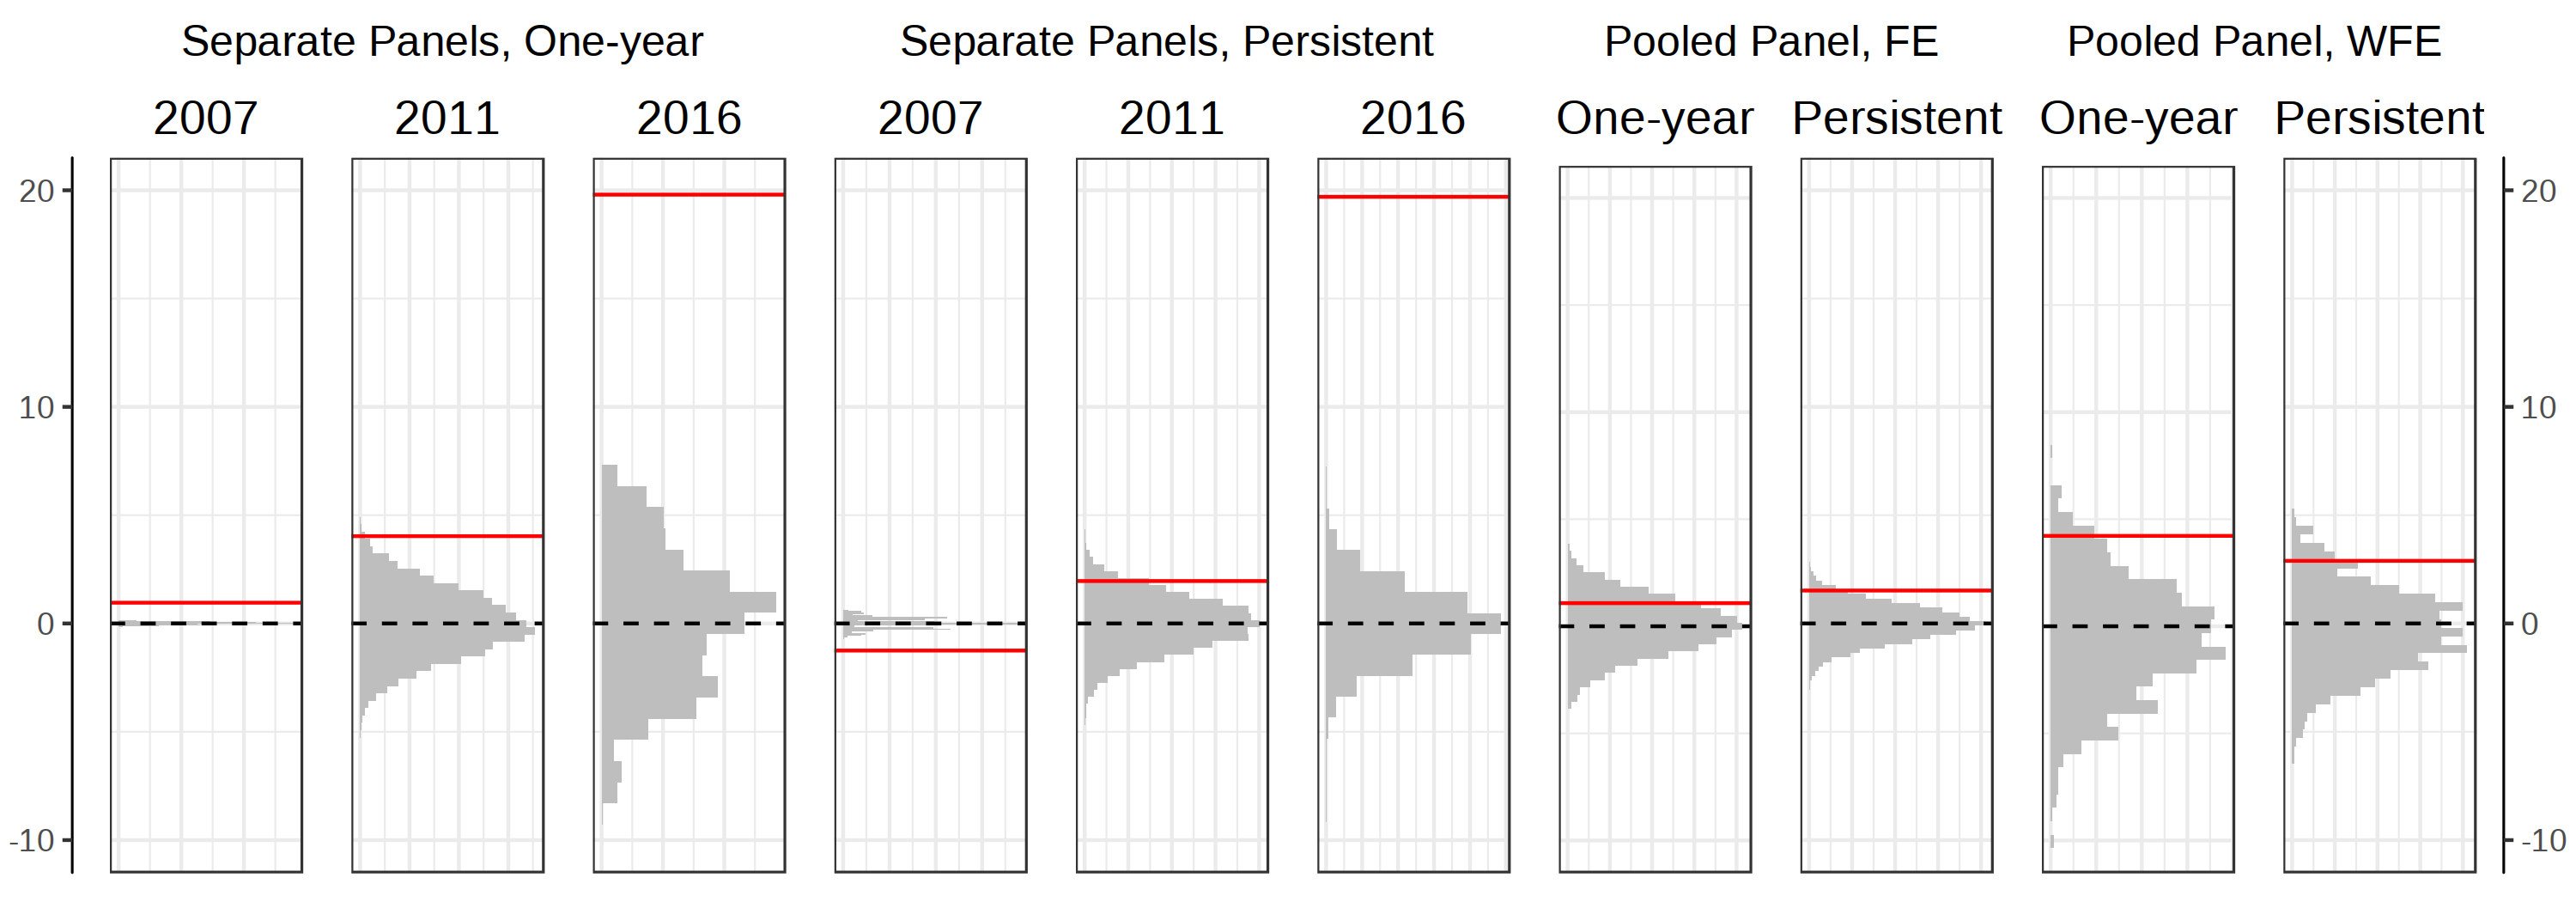
\includegraphics[width=\textwidth]{figure/SYP_FE.png}
	\captionsetup{singlelinecheck=off}
	\caption[Estimated treatment effects for linear unit fixed effects models]{Estimated treatment effects (red) and randomization distribution for linear unit fixed effects models. From left to right:
		\begin{enumerate}
			\item Cross-sectional estimate for 2007 (equation \ref{eq:FE.1})
			\item Cross-sectional estimate for 2011 (equation \ref{eq:FE.1})
			\item Cross-sectional estimate for 2016 (equation \ref{eq:FE.1})
			\item Panel estimate for 2007 (equation \ref{eq:FE.2})
			\item Panel estimate for 2011 (equation \ref{eq:FE.2})
			\item Panel estimate for 2016 (equation \ref{eq:FE.2})
			\item FE estimate, one-year effect (equation \ref{eq:FE.3})
			\item FE estimate, persistent effect (equation \ref{eq:FE.4})
			\item WFE estimate, one-year effect (WFE estimate of equation \ref{eq:FE.3})
			\item WFE estimate, one-year effect (WFE estimate of equation \ref{eq:FE.4})
		\end{enumerate}}
		\label{fig:FE}
	\end{figure}

Figure \ref{fig:FE} shows in red the estimated treatment effects for each of the linear unit fixed effect regressions in section \ref{sec:FE}, overlaid against the randomization distribution obtained by randomization inference. Overall, with the exception of only the pooled panel estimate for the contemporareous treatment effect (number 7), every estimate lies far enough to the tail of the distribution for us to reject the sharp null hypothesis. 

Among the results, the FE and WFE pooled panel estimates carry the most weight, since they make full use of the panel structure of the data. These estimates suggest a positive and statistically significant treatment effect. In other words, they show that, on average, provinces that suffered local defeats received increases in central transfer. This evidence is supportive of the theory that the CPV uses election to gather information on the geographic distribution of regime support, and interprets local defeats to be a symptom of declining support.

Between the estimates for the contemporaneous and those for persistent effects, there is no significant variation, suggesting that the increase in central transfer is quite stable. This pattern is also consistent with the above theory. Indeed, if the regime uses elections to know about the level of support in individual provinces, the only way for it to know if the buying off strategy works is to wait until the next election; until then the regime must maintain a steady flow of transfer to the province.  If instead the regime uses elections to learn about individual bureaucrats' performance, the information from elections would soon be diluted by other sources of info that the regime has, including future interactions between provincial leaders and central leadership. The bureaucrats themselves would also have opportunity to redeem themselves. This would result in a decreasing need for the regime to maintain its initial policy, which will show up in the analysis as a smaller persistent effect compared to the contemporaneous effect.

While the pooled panel estimates suggest confidence in the geographic distribution theory, the estimates for individual election years calls for some caution. In particular, across three election years there is a large variation in the estimated effects, with estimates for 2007 and 2016 being consistently positive and significant, while the estimate for 2011 switches sign depending on which specification is employed. Of course, it is almost definitely that the cross-sectional estimates are biased for reasons discussed in section \ref{sec:FE}, which renders the negative result for 2011 invalid. However, the fact that the cross-sectional and panel estimates are still quite close for 2007 and 2016 may indicate some idiosyncrasy about the 2011 election.\footnote{One possible problem is coding error: 2011 is the only election for which I do not have an authoritative list of central nominees and had to resort to coding the central nominees indicator myself} Overall, the balance of evidence still tips heavily in favor of a positive treatment effect and the ``geographic distribution'' theory.

\subsection{Synthetic Control}

\begin{figure}[ht]
	\centering
	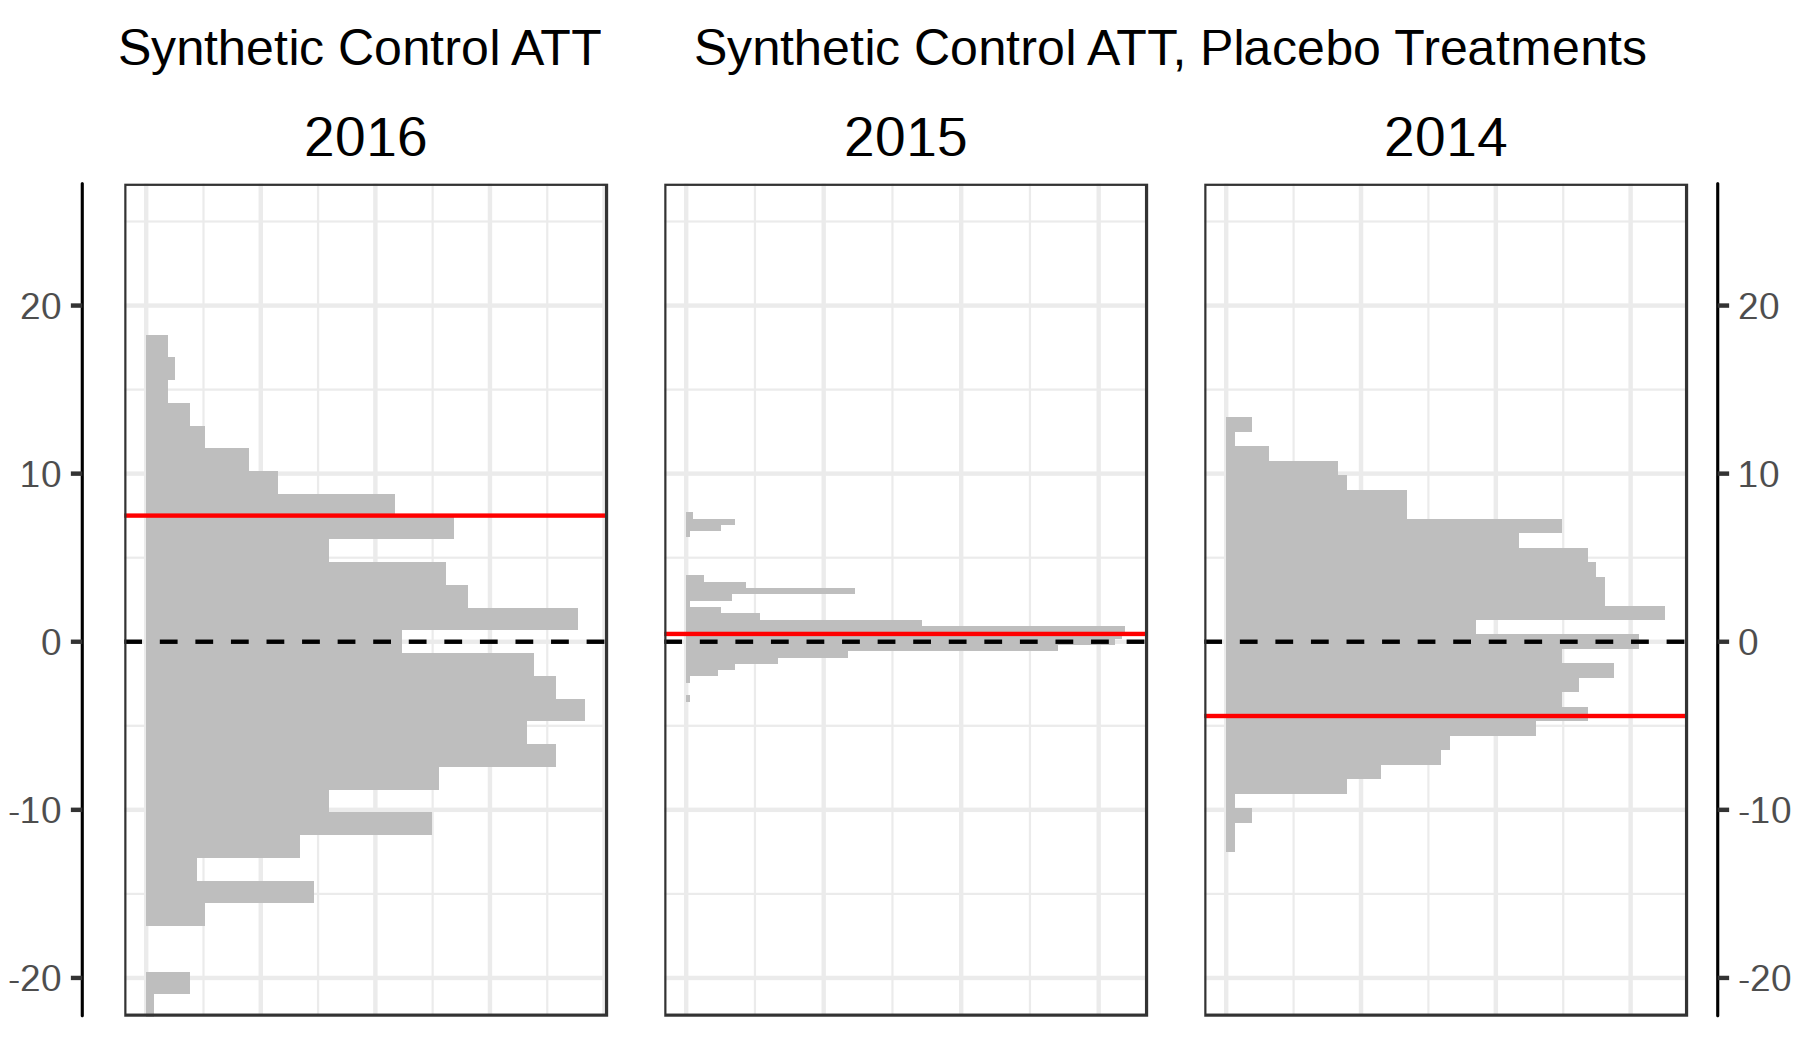
\includegraphics[width=.5\textwidth]{figure/SYP_Synth.png}
	\captionsetup{singlelinecheck=off}
	\caption[Estimated treatment effects for Synthetic Control]{Estimated treatment effect (red) and randomization distribution for synthetic control estimate for the 2016 election.}
	\label{fig:Synth}
\end{figure}

Figure \ref{fig:Synth} shows in red the estimated treatment effects for the synthetic control estimate for the 2016 election as discussed in section \ref{sec:Synth}. The treatment effect again is positive, and lies far enough to the tail of the randomization distribution ($p = 0.09$). Once again, the evidence points to an increase in central transfer to provinces that lost central nominees, thereby corroborates the `` geographic distribution'' theory and calls in question the ``local bureaucrats'' theory.

Given the discussion in section \ref{sec:vs}, it is necessary to point out that, for the 2016 election alone, the point estimate using the synthetic control method differs from both the cross-sectional and the panel estimates using fixed effects methods. The difference in magnitude is roughly 10 points on the log scale, roughly half of the fixed effects estimates. This discrepancy highlights potential violation of the causal assumption, either on the part of the fixed effects model or the synthetic control method, a problem I already noted in section \ref{sec:vs}. Considering, however, that both estimates are strongly positive and significant, it is unlikely that violation of either causal assumptions would invalidate the main conclusion of this analysis.

\section{Conclusion}
\label{sec:conclusion}

In this paper, I analyze changes in central transfer between the national government and provinces in Vietnam following three legislative elections in 2007, 2011, and 2016. Using various estimation methods to achieve causal identification, I found significant and robust evidence that the defeat of one or more central nominee(s) in a province lead to an increase in central transfer to that province. This pattern of response to local defeats is consistent with the ``geographic distribution'' theory of authoritarian election, according to which authoritarian regimes use elections to gather information about subnational variation in support for the regime, and thus corroborates this theory.

This paper, however, is not without shortcomings. To begin with, I make no pretense that its results and conclusions are generalizable to every other authoritarian regimes. What I have shown, however, is a process to identify among the many theories of authoritarian elections ones that are most applicable to each individual context, in this case the institutionalized single-party regime of Vietnam. Additionally, its conclusion rests on a chain of backward induction, each link within which is far from logically bulletproof. Finally, in terms of empirics, as the analysis in this paper shows, causal inference using non-experimental is no simple task. Even with careful measures in place, this paper still needs to rely on significant but unsubstantiated causal assumptions which have been found to be violated. 

Ultimately, however, for the modest goals it seeks to achieve, this paper does make some contribution to the larger literature. It contributes to the ``information flow'' literature of authoritarian institutions by attempting to specify the exact kind of information that authoritarian regimes collect through elections. In doing so, I evaluate two theories with potentially contradictory implications, and develop a procedure to test their validity as applied to a specific context. Throughout this paper, I conceive of authoritarian leaders as imperfect optimizers who consciously seek information to update their beliefs and modify behaviors accordingly, but are biased to interpret the information they receive in certain ways. This perspective could contribute to the broader literature on authoritarianism, which has mostly portrayed regime leaders as rational actors \citep[e.g.][]{AR2001}, by bridging it with the recent literature on political behavior which has begun to highlight the imperfect psychology of individual citizens \citep[e.g.][]{AchenBartels2016}



\bibliography{Literature/library_syp}
\end{document}
